
\chapter{Travaux de recherche} 


\section{Contexte scientifique}


\pg
Ma recherche s'inscrit dans le d\'eveloppement de SKA et ses pr\'ecurseurs, en particulier \`a basses fr\'equences. J'\'etudie l'\'evolution des galaxies et des grandes structures \`a travers les milieux inter-galactiques tels que trac\'es par le rayonnement radio-synchrotron de rayons cosmiques. Ce rayonnement subit des effets de propagation (e.g. rotation Faraday) mais n'en est pas att\'enu\'e. La radio-astronomie est donc unique car elle a pour seuls biais observationnels la qualité et maîtrise technique de leurs instruments.
La fenêtre basse-fréquence ($30-144$\,MHz) de LOFAR et NenuFAR trace les rayons cosmiques les moins énergétiques,
qui ont cess\'e d'\^etre acc\'el\'er\'es le plus longtemps avant leur d\'etection. Elle seule peut acc\`eder \`a de nombreux marqueurs cl\'es pour l'\'etude des amas de galaxies (e.g. reliques et halos radio d'amas \cite{2019SSRv..215...16V}) et de galaxies radio (e.g. bulles fossiles \cite{2021NatAs...5.1261B}). Cela n\'ecessite l'utilisation d'instruments de pointe tels que LOFAR et NenuFAR, con\c{c}us pour fournir sensibilit\'e n\'ecessaire \`a la d\'etection de ces marqueurs, et \`a la r\'esolution requise pour les \'etudier. %, mais elle est fortement impact\'ee par l'ionosph\`ere. % en 

\pg
Ma recherche se d\'eroule donc sur plusieurs axes: science des \textit{amas de galaxies} \cite[e.g.][]{2021Galax...9..105B, 2021AA...646A..56R, 2021ApJ...907...32B} et de \textit{l'\'evolution des galaxies} \cite{2022A&A...658A..10B, 2022A&A...663A..44K}, mais aussi \textit{instrumentation, mod\'elisation et algorithmes} \cite{2020AA...637A..51B, 2018AA...615A..66B} permettant \`a chaque fois de d\'epasser l'\'etat de l'art actuel pour atteindre les objectifs de sensibilit\'e et de r\'esolution n\'ecessaire \`a mes projets de recherche, et accessibles avec les instruments existants. Cette expertise a \'et\'e mise au service de \textit{l'orientation strat\'egique de plusieurs communaut\'es scientifiques nationales}, pour le d\'eveloppement d'infrastructure de calcul SKA \cite{2022arXiv220111526T} ainsi que la d\'efinition de priorit\'es scientifiques \cite{2023arXiv231110056K}; \textit{elle est centrale} \`a plusieurs collaborations et groupes de travail d\'edi\'es \`a \textit{SKA en France et \`a l'international}.






\begin{wrapfigure}[14]{r}{0.4\textwidth}\centering
	\vspace{-2.5\baselineskip}
	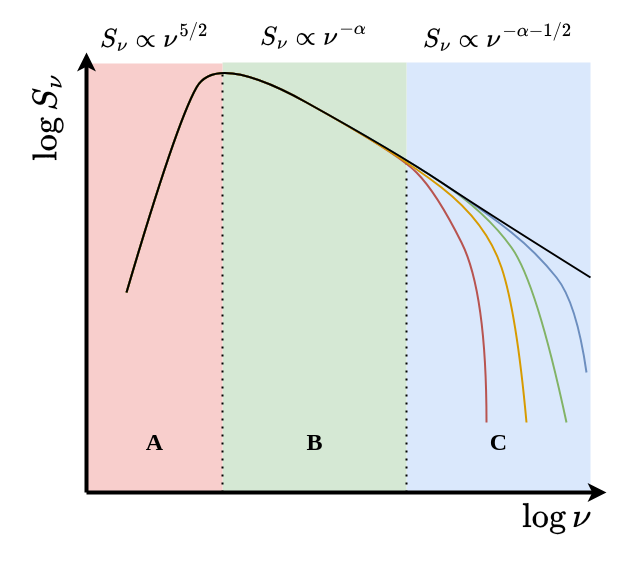
\includegraphics[width=\linewidth]{ProjetRecherche/synchrotron.drawio.png}
	\caption{Spectre synchrotron sch\'ematique.\vspace{-0.8\baselineskip}} \label{fig.synchrotron}
	\vspace{-1\baselineskip}
\end{wrapfigure}

\pg
%Mes travaux pass\'es consistent en l'\'etude du rayonnement radio-synchrotron d'objets extragalactiques \`a basses fr\'equences.
Ma recherche porte sur l'analyse du \textit{spectre} radio-synchrotron \`a basses fr\'equences. La \cref{fig.synchrotron} en r\'esume les trois r\'egimes principaux. Aux basses fr\'equences, deux comportements adviennent au-del\`a du rayonnement "classique" (r\'egime \textbf{B}), qui suit une simple loi de puissance: si le plasma devient opaque \`a l'\'emission synchrotron, celle-ci est "auto-absorb\'ee" dans sa zone d'\'emission (r\'egime \textbf{A}). Le rayonnement de rayons cosmiques acc\'el\'er\'es \`a un temps $t$ entra\^ine une perte d'\'energie, 
et donc une suppression de l'\'emission synchrotron initiale aux relativement hautes fr\'equences, en fonction de \textbf{l'\^age spectral} de cette population de rayons cosmiques (r\'egime \textbf{C}). Les basses fr\'equences sont donc la \textbf{seule fen\^etre observationelle} pour d\'etecter plusieurs types d'\'emissions fossiles.%, et ainsi contraindre l'histoire de divers objets dans l'Univers.



\pg
Il y a deux int\'er\^ets \`a \'etudier ce rayonnement \`a basses fr\'equences. Le premier est de mesurer son \^age radiatif en trouvant la fr\'equence de basculement entre les r\'egimes \textbf{B} et \textbf{C}, permettant d'\'etudier directement la diffusion et la (r\'e)acc\'el\'eration des rayons cosmiques dans les milieux intergalactiques.

\begin{wrapfigure}[14]{r}{0.35\textwidth}\centering
	\vspace{-2.5\baselineskip}
	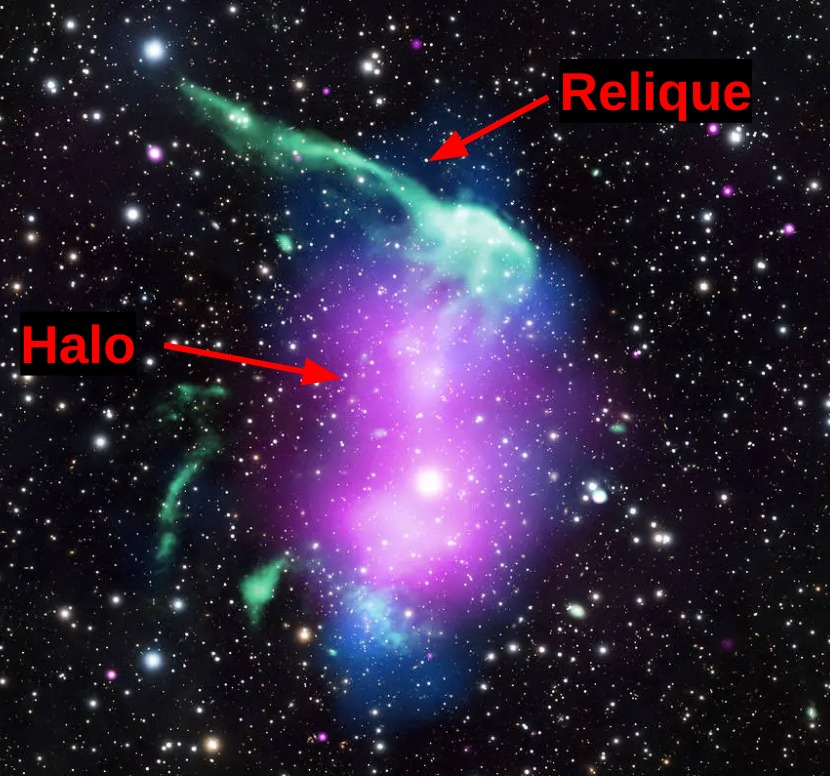
\includegraphics[width=\linewidth]{ProjetRecherche/toothbrush_edited.jpeg}
	\caption{Amas de la "brosse \`a dents"; radio en vert, X en rose. Cr\'edit image: \href{https://www.nasa.gov/wp-content/uploads/2023/03/toothbrush.jpg}{NASA}.\vspace{-0.8\baselineskip}} \label{fig.relics}
	\vspace{-.4\baselineskip}
\end{wrapfigure}


\pg
Le second int\'er\^et est de d\'etecter de nouvelles populations de rayons cosmiques fossiles, \'emettant uniquement dans le r\'egime \textbf{C}. Ils ne sont donc d\'etectables qu'\`a basses fr\'equences. %seront g\'en\'eralement pas d\'etect\'es \`a plus hautes fr\'equences, et \'evoluent dans un plasma suffisamment diffus pour que leur \'emission ne soit pas auto-absorb\'ee
L'exemple-type de ce type d'\'emission est celui des reliques radio des amas de galaxies, telles que pr\'esent\'ees dans la \cref{fig.relics}. Ces structures sont des plasma, \'eject\'es t\^ot dans le processus de formation de l'amas, qui se trouvent r\'eacc\'el\'er\'ees par des ondes de choc \`a tr\`es grande \'echelle g\'en\'er\'ees durant la formation de l'amas-h\^ote. Leur structure peut \^etre tr\`es d\'ecentr\'ee par rapport \`a l'amas, et permet alors de contraindre plusieurs sc\'enarios de formation de structure \`a grande \'echelle \cite[e.g.][]{2020AA...642L..13R}. D'autres exemples incluent la d\'etection de bulles de plasma \`a \'echelles de Mpc \cite{2021NatAs...5.1261B}. J'ai \'etudi\'e le rayonnement radio-synchrotron \`a plusieurs \'echelles: celles des amas de galaxies, des jets de galaxies, et des structures galactiques.


% sont d'un grand int\'er\^et scientifique.%pour la cosmologie observationnelle, et leur d\'etection repr\'esente une nouvelle fronti\`ere pour l'astronomie radio.
%
%\begin{tcolorbox}[colback=green!10, colframe=green!50!black, arc=3mm, boxrule=1pt]
%La sensibilit\'e des \'eclaireurs du SKA, LOFAR et NenuFAR, permet de d\'etecter de nouveaux plasmas dans des objets d\'ej\`a bien \'etudi\'es. Avec la r\'esolution angulaire de LOFAR, il est possible d'\'etudier directement les interfaces entre diff\'erents plasmas astrophysiques ainsi que la diffusion de rayons cosmiques dans ces milieux. 
%\end{tcolorbox}
%
%\newpage





\newpage
\section{Amas de galaxies}\label{pastwork.nenufar}

\pg
Mon expertise technique et scientifique a \'et\'e cl\'e dans le cadre de mon contrat post-doctoral portant sur les amas de galaxies \`a l'Universit\'e de Bologne. J'ai men\'e les d\'eveloppements instrumentaux ayant permis l'exploitation de donn\'ees ATCA \cite{2022MNRAS.515.1871R}, encadr\'e un travail de th\`ese portant sur l'\'etude d'interactions entre jet et milieu intra-amas \cite{2021A&A...650A.170B}, pr\^et\'e mon expertise \`a l'\'etude d'\'emission de ``pont'' entre composantes d'amas de galaxies \cite{2021ApJ...907...32B} et effectu\'e la \textit{premi\`ere et unique r\'eduction d\'ependante de la direction} d'observations uGMRT d'amas de galaxies \cite{2020A&A...636A..30R}. %J'ai gard\'e des liens \'etroits avec tous mes collaborateurs. 


\pg
Je suis PI du Projet Long-Terme LT09 de Nenufar, qui est la \textit{premi\`ere tentative} de d\'etecter \textbf{directement} l'\'emission radio-synchrotron provenant de filaments cosmiques. Cette d\'etection est actuellement limit\'ee par la r\'esolution angulaire de NenuFAR, qui introduit un tr\`es haut bruit de confusion (de l'ordre du Jy). L'instrument ne peux pas distinguer entre \'emission diffuse et pollution par des sources compactes. La \cref{fig.coma.nenufar} montre \textit{la limite actuellement atteignable} par NenuFAR en imagerie: la calibration des donn\'ees ne permet pas la d\'etection d'\'emission diffuse autour de l'amas de Coma, situ\'e au centre. J'ai cependant d\'etect\'e \textit{pour la premi\`ere fois \`a 60\,MHz} l'\'emission de la Boucle I du halo Galactique (le North Polar Spur), dont l'\'etendue est montr\'ee \`a droite dans la \cref{fig.coma.nenufar}. %C'est 
\begin{figure}[H]
	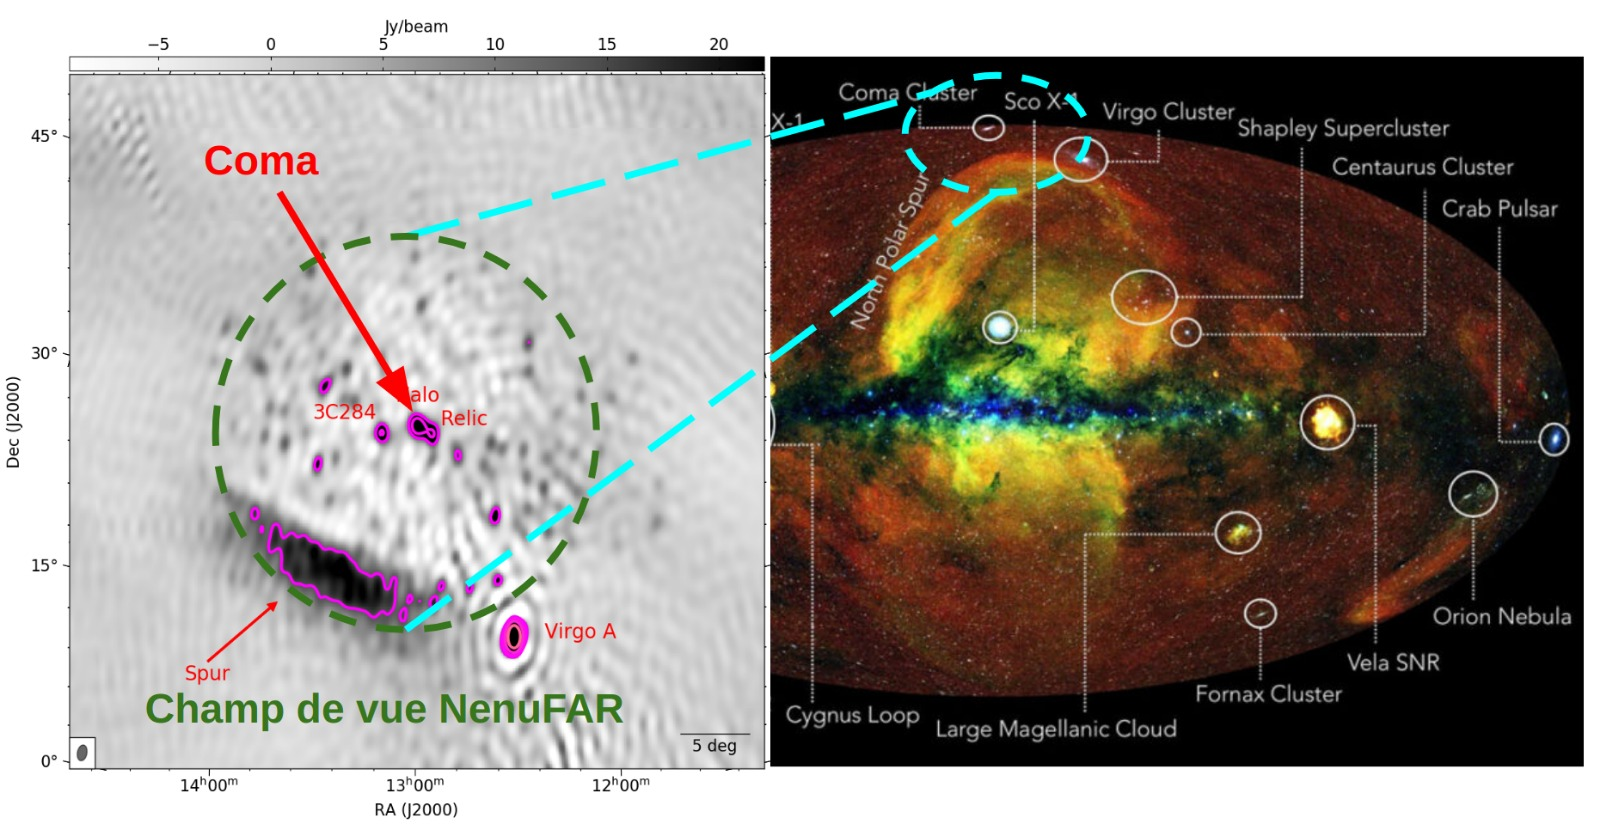
\includegraphics[width=0.96\linewidth]{ProjetRecherche/nenufar_coma.jpeg}
	\caption{\textit{Gauche}: Champ de Coma, vu par NenuFAR. \textit{Droite}: Vue eROSITA du ciel, image cr\'e\'ee par \href{https://skyandtelescope.org/astronomy-news/what-and-where-is-the-north-polar-spur/}{J. Sanders, H. Brunner \& eSASS team (MPE) / E. Churazov, M. Gilfanov (on behalf of IKI)}.} \label{fig.coma.nenufar}
\end{figure}


\pg
Je m\`ene les d\'eveloppements techniques et observationnels qui permettront de d\'epasser les limites actuelles de NenuFAR.
Ce travail n\'ecessite le d\'eveloppement et la validation de la r\'eponse instrumentale de NenuFAR sur le ciel ainsi que la calibration de l'ionosph\`ere en fonction de la direction. Ces travaux sont en cours, et seront poursuivis dans les premi\`eres phases du projet de recherche propos\'e pour cette candidature.% En 2023, j'ai pu 

\pg
Le projet LT09 de NenuFAR est un relev\'e \'eclaireur. Il se concentre sur des amas bien connus, mais descend jusqu'\`a une fr\'equence de 30\,MHz, o\`u ils n'ont encore jamais \'et\'e \'etudi\'es. Il explore donc un nouvel espace de param\`etres, m\^eme en l'absence de d\'etection directe du signal recherch\'e. Une fois finalis\'e, ce relev\'e pourra \^etre compl\'et\'e, dans sa bande haute (60\,MHz) par la soustraction de toutes \'emission compacte d\'etect\'ees par LOFAR dans le cadre de ses relev\'es LoLSS, men\'es par un co-I du projet (Francesco di Gasperin, UniBo).%Il restera 

\begin{tcolorbox}[colback=green!10, colframe=green!50!black, arc=3mm, boxrule=1pt]
	Mon expertise en imagerie NenuFAR a permis la d\'etection d'\'emission radio-synchrotron \'etendue sur de grands champs, de plusieurs degr\'es. Les développements techniques et instrumentaux que je réalise me permettent de définir la feuille de route pour la première détection directe des filaments cosmiques.
	%	 De surcro\^it, je m\`ene les d\'eveloppements techniques et instrumentaux n\'ecessaires pour am\'eliorer ces r\'esultats de pointe.
\end{tcolorbox}





\section{Galaxies radios \& Jets}

\pg
J'ai men\'e \cite{2022A&A...658A..10B}, assist\'e \cite{2022A&A...661A..92B} et encadr\'e \cite{2021A&A...650A.170B,2022A&A...663A..44K} plusieurs projets de recherche portant sur l'analyse d'interactions entre jets de galaxies radios et divers milieux inter-galactiques. Leurs r\'esultats ont pu contraindre le cycle d'activit\'e du jet galactique \cite{2022A&A...661A..92B}, d\'etecter la pr\'esence d'instabilit\'es dans le milieu inter-galactique \cite{2022A&A...661A..92B}, estimer le travail m\'ecanique effectu\'e par le jet en creusant le milieu inter-amas \cite{2021A&A...650A.170B}, ou encore contraindre l'extinction CMB dans des blazars distants \cite{2022A&A...663A..44K}. Mon projet principal sur ces interactions \cite{2022A&A...658A..10B} a port\'e sur l'analyse spectrale de 3C295 \`a 2 paires de fr\'equences. 
3C295 est une des galaxies radio les plus \'etudi\'ees dans le ciel radio, initialement recens\'ee dans le relev\'e 3C \cite{1959MmRAS..68...37E}. Je montre sa distribution de flux \`a 8.5\,GHz et 144\,MHz dans la \cref{fig.3C295}. Elle est associ\'ee \`a une galaxie-h\^ote massive de type cD \cite{1981ApJ...251..485M}, ayant $z=0.461$ \cite{2013yCat.5139....0A}. Son spectre int\'egr\'e est connu de la bande radio \cite{1990MNRAS.244..362A,1991AJ....101.1623P, 1983IEEEP..71.1295N,2011ApJ...739L...1P} \`a l'optique \cite[e.g.][]{1994A&A...285..785T} et jusqu'aux rayons X \cite[e.g.][]{2000ApJ...530L..81H,2001A&A...372..755B}. Elle sert de chandelle standard pour la calibration radio \cite{2012MNRAS.423L..30S,2017ApJS..230....7P} gr\^ace \`a son haut flux int\'egr\'e (90.87 Jy \`a 144\,MHz, 19.42 Jy \`a 1.5\,GHz) et sa compacit\'e, (\'etendue angulaire maximale $6^{\prime\prime}$). Cette compacit\'e sugg\`ere une interaction entre 3C295 et son environnement.%, particuli\`erement dans son lobe Sud.%, qui a une extension du flux radio-synchrotron semblant d\'ecouler du lobe, vers l'Est. 


\vspace{-0.5cm}

\begin{figure*}[h!]
	\centering
	\begin{subfigure}{.3\textwidth}
		\includegraphics[width=\linewidth]{ProjetRecherche/3C295_martin_flux.png}
		%\caption{3C295 r\'esolu par le VLA \`a 8.5\,GHz. PI M. Hardcastle.  \vspace{-0.8\baselineskip}} \label{fig.3c295.martin}
	\end{subfigure}
	\hfill	
	\begin{subfigure}{.3\textwidth}
		\vspace{0.45cm}
		\includegraphics[width=\linewidth]{ProjetRecherche/ccplot_boxes_reg.png}
		%\caption{Distribution de flux de 3C295 \`a 144\,MHz, avec r\'egions d'analyse spectrale.}
		\label{fig.ccplot.diag}
	\end{subfigure}
	\hfill
	\begin{subfigure}{.35\textwidth}
		\vspace{0.3cm}
		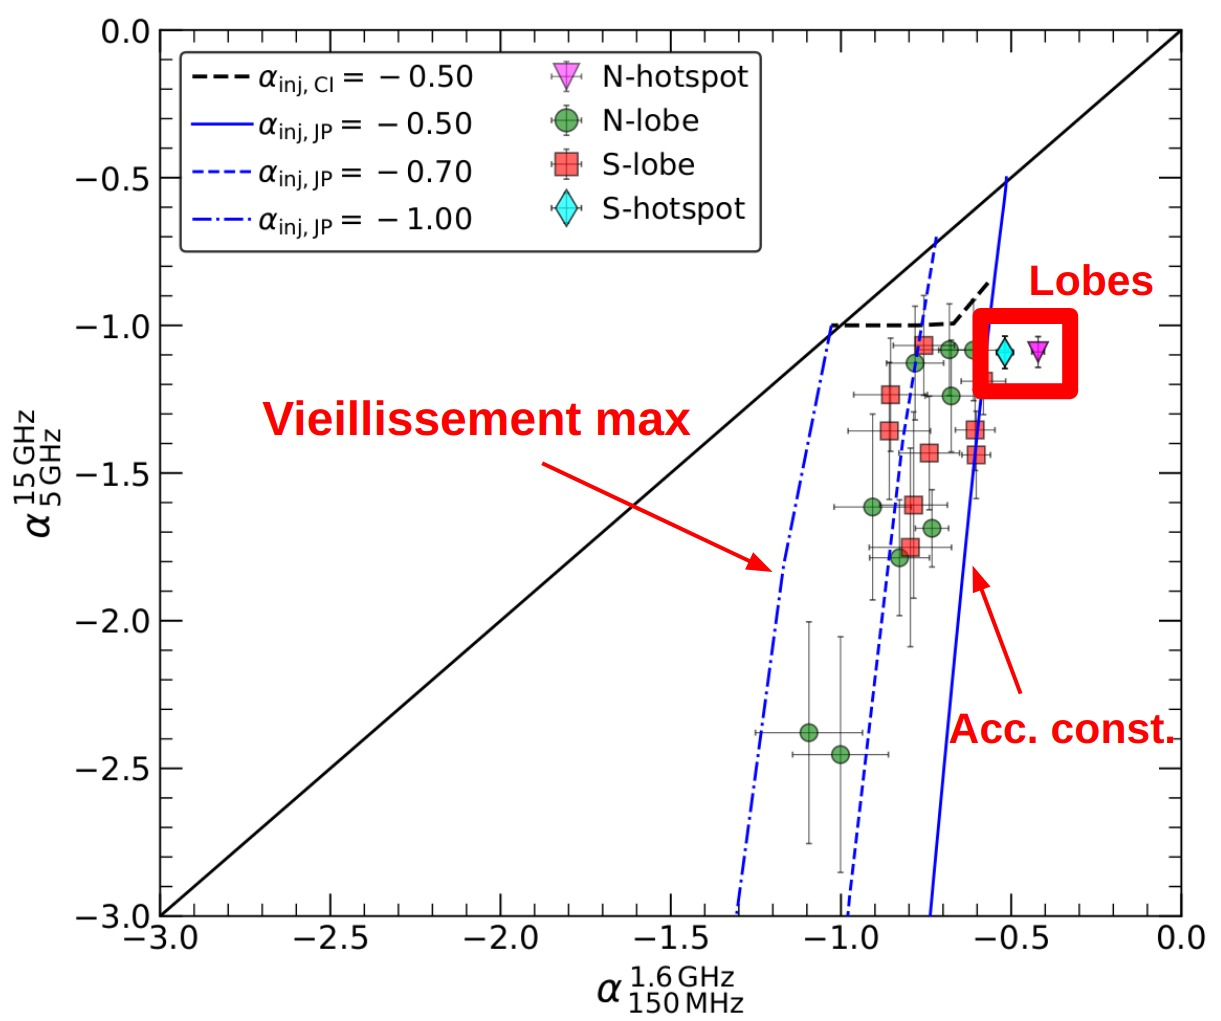
\includegraphics[width=\linewidth]{ProjetRecherche/avg_all_ccplot_annotated.jpeg}
		%\caption{Diagramme couleur-couleur radio \cite{1997ApJ...479..258K}, par r\'egion, de l'\'emission d\'etect\'ee.}
		%\label{fig.3c295.ccplot}
	\end{subfigure}
	\hfill
	\caption{\textbf{Gauche}: 3C295 vu par le VLA \`a 8.5\,GHz  (cr\'edit: M. Hardcastle. \textbf{Centre}: 3C295 vu par LOFAR-VLBI \`a 144\,MHz). \textbf{Droite}: Courbure spectrale dans les r\'egions de 3C295 identifi\'ees dans la figure centrale.}
	\label{fig.3C295}	
\end{figure*}

%\begin{wrapfigure}{r}{0.4\textwidth}\centering
%	\vspace{-4.5\baselineskip}
%	\includegraphics[width=\linewidth]{3C295_martin_flux.png}
%	\caption{3C295 r\'esolu par le VLA \`a 8.5\,GHz. PI M. Hardcastle.  \vspace{-0.8\baselineskip}} \label{fig.3c295.martin}
%	\vspace{-0.8\baselineskip}
%\end{wrapfigure}
%
%
%\begin{wrapfigure}{r}{0.4\textwidth}\centering
%	\vspace{-2.0\baselineskip}
%	\includegraphics[width=\linewidth]{ccplot_boxes_reg.png}
%	\caption{Distribution de flux de 3C295 \`a 144\,MHz, avec r\'egions d'analyse spectrale.}
%	\vspace{-0.8\baselineskip}
%\end{wrapfigure}




\pg
Mon analyse montre que le spectre des rayons cosmiques change de courbure en fonction de leur diffusion dans le milieu intergalactique. Bien que LOFAR aie une r\'esolution inf\'erieure au VLA, il d\'etecte de nouvelles r\'egions d'\'emission. La couverture spectrale disponible n'a pas permis d'estimer la fr\'equence limite entre les r\'egimes synchrotrons \textbf{B} et \textbf{C}, mais montre que les courbures spectrales des lobes ne sont pas compatible avec une seule acc\'el\'eration mais plut\^ot une \textbf{absorption} \`a 144\,MHz (r\'egime \textbf{A} de \cref{fig.synchrotron}). Ces r\'esultats sont montr\'es en \cref{fig.3C295} \cite{2022A&A...658A..10B}. 
La majorit\'e de l'\'emission d\'etect\'ee est compatible avec un mod\`ele radiatif de type KP/JP , c'est-\`a-dire 1 acc\'el\'eration puis rayonnement, \cite{1973A&A....26..423J}. Elle est donc localis\'ee dans la r\'egion entre les lignes de la figure de droite de \cref{fig.3C295}. La courbure spectrale mesur\'ee dans les lobes sort de cette r\'egion. Elle est donc compatible avec tout sc\'enario d'acc\'eleration-puis-\'emission: injection continue, \'emission Jaffe-Perola \cite{1973A&A....26..423J}, \'emission Kardashev-Perola \cite{1962SvA.....6..317K}. Ces lobes sont donc opaques au rayonnement synchrotron \`a basses fr\'equences. \textit{Il n'y a pas d'acc\'el\'eration locale de rayons cosmiques aux terminus des jets de 3C295: ce ne sont pas des zones de choc.} Les rayons cosmiques diffus\'es dans le milieu inter-galactique autour de 3C295 n'ont donc \'et\'e acc\'el\'er\'es que dans le jet.
% Les lobes ont une courbure spectrale qui n'est compatible ni avec ce mod\`ele, ni une r\'eacc\'el\'eration continue. Au contraire, l'indice spectral des basses fr\'equences est trop plat, et celui vers les hautes fr\'equences trop pentu. Le milieu intergalactique est opaque aux lobes, \`a basses fr\'equences, et redevient optiquement fin une fois la diffusion du plasma dans le milieu environnant.



\begin{tcolorbox}[colback=green!10, colframe=green!50!black, arc=3mm, boxrule=1pt]
	Mon expertise en analyse spectrale du rayonnement radio-synchrotron me permet d'analyser les interactions entre jets galactiques et divers milieux environnants, allant des amas de galaxies aux groupes, en identifiant les propri\'et\'es des rayons cosmiques ainsi que des milieux dans lesquels ils rayonnent.
\end{tcolorbox}

\begin{tcolorbox}[colback=green!20, colframe=green!50!black, arc=3mm, boxrule=2pt]
	Ce sujet est directement reli\'e \`a la th\'ematique de recherche du poste pour lequel je candidate. \`A l'heure actuelle, de tr\`es nombreuses sources radio d\'etect\'ees par LOFAR n'ont pas d'information de redshift; des projets tels que \href{https://ingconfluence.ing.iac.es/confluence/display/WEAV/WEAVE-LOFAR}{WEAVE-LOFAR} {\oe}uvrent \`a acqu\'erir cette information critique. \textbf{Avec le JWST, il sera possible d'associer directement \`a ces sources leurs contreparties d\'etect\'ees dans les relev\'es grand-champs de LOFAR, MeerKAT, et le futur SKA}. De nouveaux seuils de sensibilit\'e radio devront \^etre franchis: \textbf{je participe activement aux travaux qui rendront cela possible}.
\end{tcolorbox}




\newpage







\section{Les milieux galactiques}

\pg
Une partie importante de mon travail depuis 2021, en collaboration avec Fran\c{c}oise Combes (LERMA-OBSPM), Anne-Laure Melchior (LERMA-OBSPM) et Cyril Tasse (GEPI-OBSPM), porte sur l'\'etude des champs magn\'etiques intra-galactiques, et la diffusion des rayons cosmiques dans ces milieux. L'origine et la diffusion des rayons cosmiques au sein des galaxies est une question encore ouverte. Les champs magn\'etiques galaxiques peuvent se diviser en trois composantes principales: \textbf{I}. les champs \textit{ordonn\'es}, dans lesquels l'\'emission radio-synchrotron sera polaris\'ee, et qui s'alignent avec les structures dominantes d'une galaxie (e.g. "bras magn\'etiques" entre bras optiques de galaxies spirales, cf \cite{1996NAWG.1996..262B}); \textbf{II. } les champs \textit{turbulents isotropes}, g\'en\'er\'es par des ph\'enom\`nes comme les restes de supernovae; et \textbf{III.} les champs \textit{turbulents anisotropes}, g\'en\'er\'es des champs turbulents isotropes par compression ou flux de cisaillement. Selon la taille de la galaxie \cite{2009A&A...494...21A}, des effets de dynamo large-\'echelle peuvent g\'en\'erer, sur des \'echelles de temps de Gyr, un champ r\'egulier \cite{1988ASSL..133.....R}. Les champs ordonn\'es et r\'eguliers jouent un r\^ole important dans le confinement et la diffusion de rayons cosmiques  \cite{2013PhPl...20e5501Z}, mais aussi dans l'\'evolution de la galaxie en contrant l'effet du potentiel gravitationnel sur le gaz \cite{1990ApJ...365..544B}, participant au refroidissement du milieu interstellaire, et contenant les \'ecoulements de supernovae \cite{2019MNRAS.488.5065E}. Les champs magn\'etiques jouent aussi un r\^ole dans la formation stellaire \cite{2019FrASS...6....7K}.

%
%
%\begin{wrapfigure}{r}{0.4\textwidth}\centering
%	\vspace{-1.2\baselineskip}
%	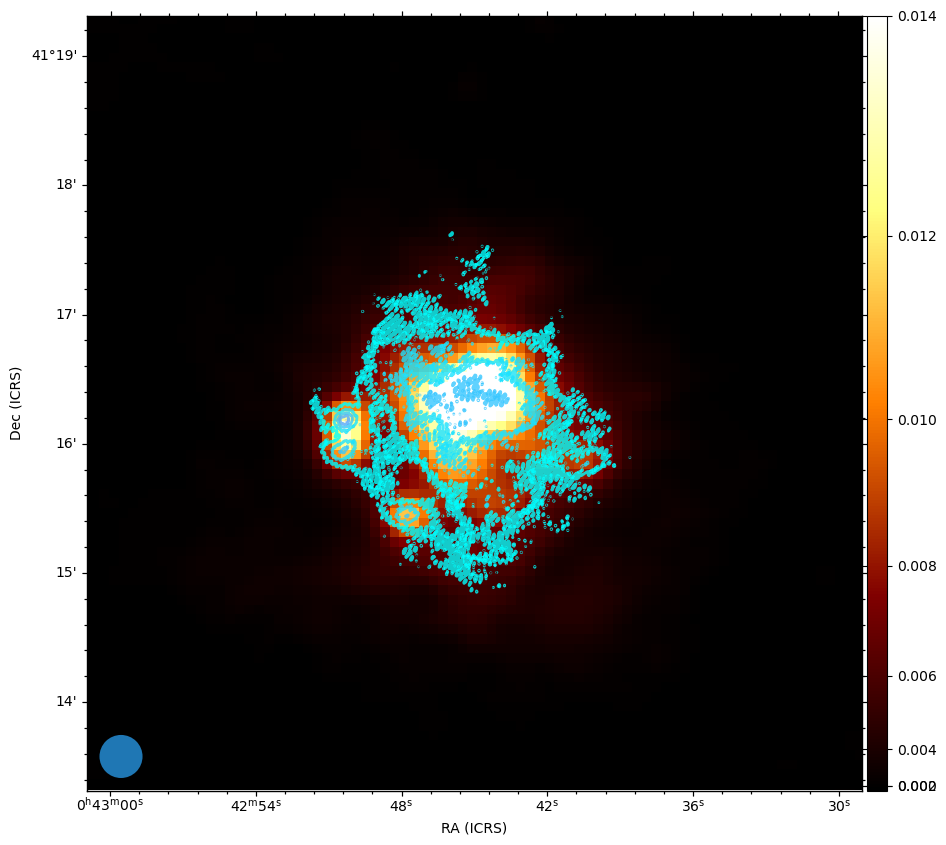
\includegraphics[width=\linewidth]{M31-lowres-LOFAR.fits.png}
%	\caption{Image couleur: zoom de l'image de \cref{fig.m31.lofar.nenufar}, centr\'e sur le c{\oe}ur d'Androm\`ede. Contours: distribution de flux avec LOFAR-VLBI. On distingue le d\'ebut des bras de spirale de la galaxie, ainsi que la pr\'esence de noeuds en leurs sein. \vspace{-0.8\baselineskip}} \label{fig.m31.core.vlbi}
%	\vspace{-0.8\baselineskip}
%\end{wrapfigure}




\pg
Je travaille donc avec Anne-Laure Melchior et Fran\c{c}oise Combes (LERMA-OBSPM), ainsi que Cyril Tasse (GEPI-OBSPM),  sur la r\'eduction de donn\'ees LOFAR, y compris ses stations internationales, ciblant la galaxie d'Androm\`ede (PI: Anne-Laure Melchior). Cyril Tasse a initialement calibr\'e ces donn\'ees \`a une r\'esolution de $5''$. J'ai r\'eussi la calibration initiale \`a r\'esolution de $0.4''$ en \'et\'e 2023. \textit{J'ai pu, pour la premi\`ere fois, cr\'eer une image LOFAR-VLBI d'un champ aussi complexe.} De nombreux effets de calibration restent \`a r\'esoudre dans le champ, mais les milieux de cette galaxie dans son ensemble sont d\'esormais accessibles avec une r\'esolution de dizaines de parsecs. La \cref{fig.andromeda} montre Androm\`ede vue par NenuFAR, LOFAR et avec le LOFAR-VLBI: il ne reste plus qu'\`a r\'eduire les donn\'ees LOFAR \`a 60\,MHz pour compl\'eter la couverture basses-fr\'equences d'Androm\`ede, permettant d'\'etudier les champs magn\'etiques et populations de rayons cosmiques fossiles dans son champ. Ce travail est donc id\'eal pour tisser des liens entre les futurs P\^oles de recherche de l'Observatoire.

\begin{figure}[H]
	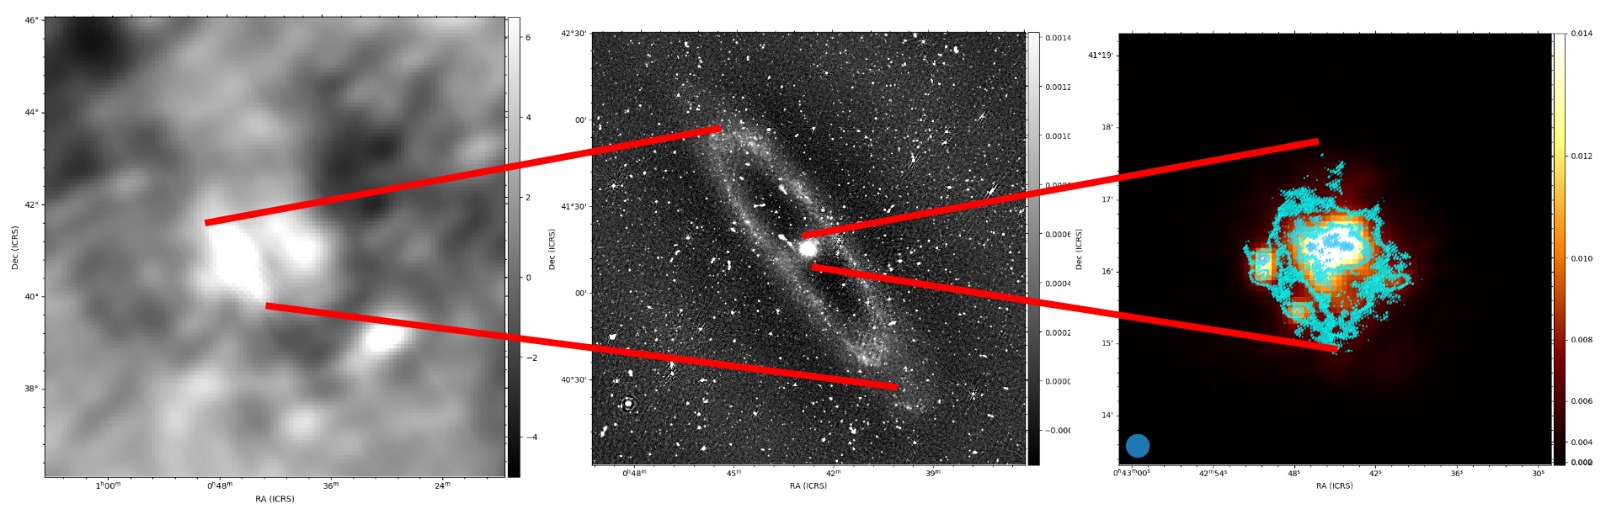
\includegraphics[width=\linewidth]{ProjetRecherche/andromeda-full.jpeg}
	\caption{Gauche: Androm\`ede vu par NenuFAR. Centre: Androm\`ede avec LOFAR. Droite: Superposition de LOFAR-VLBI sur le c{\oe}ur d'Androm\`ede tel que vu par LOFAR.} \label{fig.andromeda}
\end{figure}

\pg
Fort de ce succ\`es, j'ai obtenu 10h d'observations NenuFAR, et 32h d'observation LOFAR-LBA (sans stations internationales) sur ce m\^eme champ. J'ai men\'e \`a bien la calibration des donn\'ees NenuFAR, en attendant les donn\'ees LOFAR qui seront prises en \'et\'e 2024. \textit{Les techniques d\'eploy\'ees dans le contexte de ce travail r\'esultent d'un v\'eritable travail de recherche technique et observationnel dont je suis le moteur.} Les fruits de ce travail sont g\'en\'eralisables \`a d'autres projets, dont celui propos\'e dans le cadre de ma candidature.

%
%\begin{figure}[h!]
%	
%	\centering
%	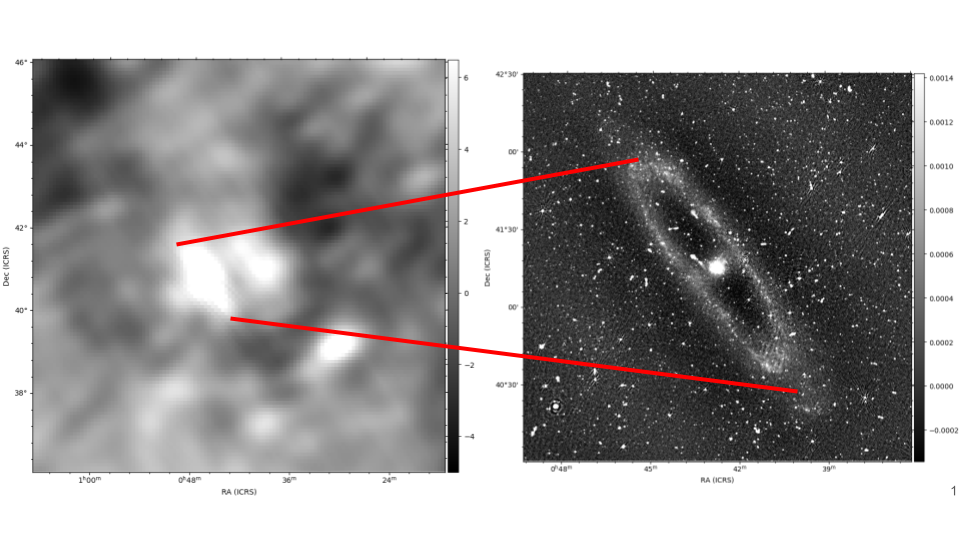
\includegraphics[width=0.8\linewidth]{M31_lofar_nenufar.png}
%	\caption{\textbf{Gauche}: distribution de flux mesur\'ee par NenuFAR \`a 60\,MHz dans le champ d'Androm\`ede. \textbf{Droite}: distribution de flux mesur\'ee \`a 144\,MHz par LOFAR; le halo elliptique de formation d'\'etoiles est clairement visible. \`A noter que NenUFAR n'est pas capable de distinguer entre flux diffus et 'nuages' de sources compactes, visibles dans l'image LOFAR.} \label{fig.m31.lofar.nenufar}
%\end{figure}

\begin{tcolorbox}[colback=green!10, colframe=green!50!black, arc=3mm, boxrule=1pt]
	Je suis le premier expert LOFAR-VLBI \`a cr\'eer une image LOFAR-VLBI grand-champ d'une galaxie proche. Je m\`ene le d\'eveloppement de nouveaux modes d'utilisation des observations LOFAR et NenuFAR afin d'\'etudier simultan\'ement l'\'emission aux plus grandes et aux plus petites \'echelles. Je fais ainsi d'une pierre deux coups: je permets l'analyse de toutes les sources compactes dans mes champs observ\'es, et je soustrais optimalement leur \'emission dans ma recherche d'\'emission diffuse sous-jacente.
\end{tcolorbox}

